\documentclass[../main.tex]{subfiles}
\begin{document}
\counterwithin{figure}{section}
\counterwithin{table}{section}
\section{Additional tables}




%\begin{landscape}
\begin{table}[H]
    \centering
    \caption{Balance test (native)}
    \label{tab:balance_test_native_full}
    \begin{adjustbox}{width = \linewidth, center}
    \begin{threeparttable}
        \begin{tabular}[t]{lccccccc}
\toprule
  & Income (1,000) & Net wealth (1,000) & Oldest HH member (years) & Tenure (days) & Employed & Educ. length (years) & HH size\\
\midrule
New diff neighbor $k_{nearest}$ v $k_{near}$ & -1.408*** & -1.903*** & -0.043* & 1.936 & -0.002** & -0.035* & -0.009***\\
 & (0.254) & (0.402) & (0.020) & (5.999) & (0.001) & (0.014) & (0.002)\\
New diff neighbor $k_{near}$ v $k_{near}$ (omit.) &  &  &  &  &  &  & \\
 &  &  &  &  &  &  & \\
New diff neighbor $k_{close,10}$ v $k_{near}$ & -0.042 & 0.620 & 0.031 & 20.750*** & 0.001 & 0.010 & 0.005*\\
 & (0.255) & (0.402) & (0.019) & (5.710) & (0.001) & (0.013) & (0.002)\\
New diff neighbor $k_{close,20}$ v $k_{near}$ & 0.498* & 1.625*** & 0.109*** & 53.312*** & 0.002** & 0.025* & 0.015***\\
 & (0.224) & (0.377) & (0.018) & (5.262) & (0.001) & (0.013) & (0.002)\\
New diff neighbor $k_{close,30}$ v $k_{near}$ & 1.429*** & 2.993*** & 0.228*** & 93.723*** & 0.005*** & 0.045** & 0.029***\\
 & (0.256) & (0.402) & (0.019) & (5.823) & (0.001) & (0.014) & (0.003)\\
New diff neighbor $k_{close,40}$ v $k_{near}$ & 1.805*** & 4.979*** & 0.343*** & 124.422*** & 0.004*** & 0.055*** & 0.040***\\
 & (0.307) & (0.496) & (0.023) & (7.935) & (0.001) & (0.016) & (0.003)\\
\midrule
N & 5,365,811 & 5,365,811 & 5,365,811 & 5,365,811 & 5,365,811 & 5,365,811 & 5,365,811\\
Neighborhood-by-quarter FE & X & X & X & X & X & X & X\\
Mean of dependent variable & 341.26 & 60.61 & 44.05 & 2646.87 & 0.84 & 10.11 & 1.70\\
Number of neighborhoods & 3444 & 3444 & 3444 & 3444 & 3444 & 3444 & 3444\\
\bottomrule
\end{tabular}
    \begin{tablenotes}[flushleft]
    \item \scriptsize * p < 0.05, ** p < 0.01, *** p < 0.001. Standard errors (in parenthesis) are clustered at the neighborhood level. The table reports the estimate of $\phi_k - \phi_2$ from equation \ref{eq:main_eq_schelling_behavior} for each distance band $k$, for $k\in {[1-3], [7-10], [11-20], [21-30], [31-40]}$ from equation \ref{eq:balance_tests}. 
    \end{tablenotes}
    \end{threeparttable}
    \end{adjustbox}
\end{table}

\begin{table}[H]
    \centering
    \caption{Balance test (non-Western)}
    \label{tab:balance_test_non_west_full}
    \begin{adjustbox}{width = \linewidth, center}
    \begin{threeparttable}
        \begin{tabular}[t]{lccccccc}
\toprule
  & Income (1,000) & Net wealth (1,000) & Oldest HH member (years) & Tenure (days) & Employed & Educ. length (years) & HH size\\
\midrule
New diff neighbor $k_{nearest}$ v $k_{near}$ & -0.065 & 0.171 & -0.061* & 31.109*** & 0.001 & -0.011 & 0.001\\
 & (0.347) & (0.522) & (0.028) & (7.656) & (0.001) & (0.018) & (0.004)\\
New diff neighbor $k_{near}$ v $k_{near}$ (omit.) &  &  &  &  &  &  & \\
 &  &  &  &  &  &  & \\
New diff neighbor $k_{close,10}$ v $k_{near}$ & -0.075 & 0.514 & 0.064* & 58.269*** & 0.002 & 0.024 & 0.026***\\
 & (0.350) & (0.507) & (0.027) & (7.448) & (0.001) & (0.017) & (0.004)\\
New diff neighbor $k_{close,20}$ v $k_{near}$ & -0.315 & 0.400 & 0.191*** & 111.810*** & 0.001 & 0.021 & 0.039***\\
 & (0.319) & (0.467) & (0.026) & (6.707) & (0.001) & (0.015) & (0.004)\\
New diff neighbor $k_{close,30}$ v $k_{near}$ & -0.760* & 1.043 & 0.297*** & 157.738*** &  & 0.030 & 0.062***\\
 & (0.348) & (0.536) & (0.028) & (7.760) & (0.001) & (0.018) & (0.005)\\
New diff neighbor $k_{close,40}$ v $k_{near}$ & -1.064* & 2.171** & 0.430*** & 202.154*** &  & 0.013 & 0.064***\\
 & (0.455) & (0.700) & (0.037) & (10.536) & (0.002) & (0.023) & (0.006)\\
\midrule
N & 1,795,109 & 1,795,109 & 1,795,109 & 1,795,109 & 1,795,109 & 1,795,109 & 1,795,109\\
Neighborhood-by-quarter FE & X & X & X & X & X & X & X\\
Mean of dependent variable & 315.64 & 46.50 & 42.94 & 2298.84 & 0.84 & 12.11 & 2.11\\
Number of neighborhoods & 3,332 & 3,332 & 3,332 & 3,332 & 3,332 & 3,332 & 3,332\\
\bottomrule
\end{tabular}
    \begin{tablenotes}[flushleft]
    \item \scriptsize * p < 0.05, ** p < 0.01, *** p < 0.001. Standard errors (in parenthesis) are clustered at the neighborhood level. The table reports the estimate of $\phi_k - \phi_2$ from equation \ref{eq:main_eq_schelling_behavior} for each distance band $k$, for $k\in {[1-3], [7-10], [11-20], [21-30], [31-40]}$ from equation \ref{eq:balance_tests}.  
    \end{tablenotes}
\end{threeparttable}
\end{adjustbox}
\end{table}
%\end{landscape}

\begin{table}[H]
    \caption{Estimate of Schelling behavior (native households)}
    \label{tab:main_results_full}
    \centering
    \begin{threeparttable}
        \begin{tabular}{lcccc}
\toprule
  & (1) & (2) & (3) & (4) \\ 
\midrule
New diff-type neighbor $k_{nearest}$ v $k_{close,20}$ & 0.949*** & 0.962*** & 0.747*** & 0.702*** \\ 
 & (0.097) & (0.098) & (0.090) & (0.077) \\ 
New diff-type neighbor $k_{near}$ v $k_{close,20}$ & 0.599*** & 0.601*** & 0.400*** & 0.379*** \\ 
 & (0.052) & (0.054) & (0.057) & (0.059) \\ 
New diff-type neighbor $k_{close,10}$ v $k_{close,20}$ & 0.331*** & 0.333*** & 0.220** & 0.201** \\ 
 & (0.067) & (0.067) & (0.068) & (0.070) \\ 
New diff-type neighbor $k_{close ,20}$ v $k_{close ,20}$ (omitted) &  &  &  & \\ 
 &  &  &  &  \\ 
New diff-type neighbor $k_{close,30}$ v $k_{close,20}$ & -0.765*** & -0.771*** & -0.674*** & -0.623*** \\ 
 & (0.047) & (0.047) & (0.046) & (0.042) \\ 
New diff-type neighbor $k_{close,40}$ v $k_{close,20}$ & -1.528*** & -1.537*** & -1.435*** & -1.327*** \\ 
 & (0.141) & (0.142) & (0.140) & (0.135) \\ 
Income 200,000 DKK - 400,001 DKK (omitted) &  & & & \\ 
 &  & & & \\ 
Income 400,001 DKK - 600,000 DKK &  & 1.829*** & 1.772*** & 1.989*** \\ 
 &  & (0.186) & (0.163) & (0.218) \\ 
Income 600,001 DKK - 800,000 DKK &  & 4.181*** & 3.621*** & 4.110*** \\ 
 &  & (0.285) & (0.246) & (0.348) \\ 
Income 800,001 DKK - 1,000,000 DKK &  & 5.557*** & 4.578*** & 5.706*** \\ 
 &  & (0.331) & (0.375) & (0.469) \\ 

Tenure $<1$ year (omitted) &  &  &  &  \\ 
 &  &  &  & \\ 

Tenure $[1-2[$ years &  &  & -2.840*** & -2.750*** \\ 
 &  &  & (0.350) & (0.336) \\ 
Tenure $[2-4[$ years &  &  & -6.540*** & -6.225*** \\ 
 &  &  & (0.386) & (0.377) \\ 
Tenure $[4-6[$ years &  &  & -10.189*** & -9.493*** \\ 
 &  &  & (0.329) & (0.335) \\ 
Tenure $\geq$ 6 years &  &  & -18.000*** & -14.715*** \\ 
 &  &  & (0.388) & (0.323) \\ 

 
Oldest in HH, age 30-40 (omitted) &  &  &  & \\ 
 &  &  &  & \\ 

 
Oldest in HH, age 41-50 &  &  &  & -9.385*** \\ 
 &  &  &  & (0.604) \\ 
Oldest in HH, age 51-60 &  &  &  & -12.828*** \\ 
 &  &  &  & (0.472) \\ 
\midrule
N & 5,369,040 & 5,369,040 & 5,369,040 & 5,369,040 \\ 
Neighborhood-by-quarter FE & X & X & X & X \\ 
Mean of dependent variable & 20.16 & 20.16 & 20.16 & 20.16 \\ 
Number of neighborhoods & 3443 & 3443 & 3443 & 3443 \\ 
Income &  & X & X & X \\ 
Tenure &  &  & X & X \\ 
Age &  &  &  & X \\ 
\bottomrule
\end{tabular}
    \begin{tablenotes}[flushleft]
    \item \scriptsize * p < 0.05, ** p < 0.01, *** p < 0.001. Standard errors (in parenthesis) are clustered at the neighborhood level. The table reports the estimate of $\beta_k - \beta_2$ from equation \ref{eq:main_eq_schelling_behavior} for each distance band $k$, for $k\in {[1-3], [7-10], [11-20], [21-30], [31-40]}$. 
    \end{tablenotes}
    \end{threeparttable}
\end{table}

\begin{table}[H]
    \caption{Estimate of Schelling behavior (non-Western households)}
    \label{tab:main_results_full_non_west}
    \centering
    \begin{threeparttable}
        \begin{tabular}{lcccccc}
\toprule
 & \multicolumn{6}{c}{Move within 2 years (=100)} \\ 
\cmidrule(lr){2-7}
 & \multicolumn{6}{c}{<=25m} \\ 
\cmidrule(lr){2-7}
  & (1) & (2) & (3) & (4) & (5) & (6) \\ 
\midrule
New diff neighbor $k_{nearest}$ v $k_{near}$ & 0.063 & 0.062 & 0.155 & 0.097 & 0.097 & 0.096 \\ 
 & (0.129) & (0.129) & (0.127) & (0.126) & (0.126) & (0.126) \\ 
New diff neighbor $k_{near}$ v $k_{near}$ (omit.) & & & & & & \\ 
 &   &   &   &   &   &   \\ 
New diff neighbor $k_{close,10}$ v $k_{near}$ & -0.381** & -0.384** & -0.154 & -0.160 & -0.159 & -0.161 \\ 
 & (0.125) & (0.125) & (0.121) & (0.120) & (0.120) & (0.120) \\ 
New diff neighbor $k_{close,20}$ v $k_{near}$ & -0.715*** & -0.716*** & -0.307** & -0.272* & -0.269* & -0.271* \\ 
 & (0.115) & (0.115) & (0.112) & (0.111) & (0.111) & (0.111) \\ 
New diff neighbor $k_{close,30}$ v $k_{near}$ & -1.294*** & -1.292*** & -0.735*** & -0.674*** & -0.673*** & -0.673*** \\ 
 & (0.122) & (0.122) & (0.117) & (0.116) & (0.116) & (0.116) \\ 
New diff neighbor $k_{close,40}$ v $k_{near}$ & -2.009*** & -2.003*** & -1.321*** & -1.214*** & -1.215*** & -1.212*** \\ 
 & (0.143) & (0.143) & (0.135) & (0.131) & (0.131) & (0.131) \\ 
 Income 200,000 DKK - 400,000 DKK (omit.) &  &  &  &  &  &  \\ 
 &  &  &  &  &  &  \\ 
 Income 400,001 DKK - 600,000 DKK &  & 1.464*** & 1.268*** & 0.962*** &  & 1.054*** \\ 
 &  & (0.186) & (0.174) & (0.171) &  & (0.170) \\ 
Income 600,001 DKK - 800,000 DKK &  & 3.955*** & 3.055*** & 2.434*** &  & 2.627*** \\ 
 &  & (0.446) & (0.423) & (0.417) &  & (0.416) \\ 
Income 800,001 DKK - 1,000,000 DKK &  & 7.488*** & 6.284*** & 5.867*** &  & 6.124*** \\ 
 &  & (0.879) & (0.869) & (0.845) &  & (0.846) \\ 
 Tenure $<1$ year (omit.) &  &  &  &  &  &  \\ 
 &  &  &  &  &  &  \\ 
 Tenure $[1-2[$ years &  &  & -3.216*** & -3.012*** & -3.001*** & -3.007*** \\ 
 &  &  & (0.189) & (0.187) & (0.187) & (0.187) \\ 
Tenure $[2-4[$ years &  &  & -7.436*** & -6.769*** & -6.759*** & -6.753*** \\ 
 &  &  & (0.219) & (0.219) & (0.219) & (0.219) \\ 
Tenure $[4-6[$ years &  &  & -11.126*** & -9.747*** & -9.741*** & -9.722*** \\ 
 &  &  & (0.241) & (0.240) & (0.240) & (0.240) \\ 
Tenure $\geq 6$ years &  &  & -17.234*** & -13.162*** & -13.195*** & -13.145*** \\ 
 &  &  & (0.227) & (0.226) & (0.226) & (0.226) \\ 
Oldest in HH, age 30-40 (omit.) &  &  &  &  &  &  \\ 
 &  &  &  & &  &  \\ 
Oldest in HH, age 41-50 &  &  &  & -8.573*** & -8.593*** & -8.556*** \\ 
 &  &  &  & (0.145) & (0.145) & (0.145) \\ 
Oldest in HH, age 51-60 &  &  &  & -12.999*** & -13.045*** & -12.999*** \\ 
 &  &  &  & (0.159) & (0.159) & (0.159) \\ 
Wealth -200,000 DKK - 0 DKK (omit.) &  &  &  &  &  &  \\ 
 &  &  &  &  &  &  \\ 
 Wealth 1 - 200,000 DKK &  &  &  &  & 0.774*** & 0.770*** \\ 
 &  &  &  &  & (0.121) & (0.121) \\ 
Wealth 200,001 - 400,000 DKK &  &  &  &  & 0.772*** & 0.464* \\ 
 &  &  &  &  & (0.231) & (0.230) \\ 
Wealth 400,001 - 600,000 DKK &  &  &  &  & -0.506 & -0.936** \\ 
 &  &  &  &  & (0.293) & (0.289) \\ 
Wealth 600,001 - 750,000 DKK &  &  &  &  & -0.676 & -1.191** \\ 
 &  &  &  &  & (0.411) & (0.410) \\ 
 \midrule
N & 1,795,109 & 1,795,109 & 1,795,109 & 1,795,109 & 1,795,109 & 1,795,109 \\ 
Neighborhood-by-quarter FE & X & X & X & X & X & X \\ 
Mean of dependent variable & 19.96 & 19.96 & 19.96 & 19.96 & 19.96 & 19.96 \\ 
Number of neighborhoods & 3332 & 3332 & 3332 & 3332 & 3332 & 3332 \\ 
Income &  & X & X & X &  & X \\ 
Wealth &  &  &  &  & X & X \\ 
Tenure &  &  & X & X & X & X \\ 
Age &  &  &  & X & X & X \\ 
\bottomrule
\end{tabular}
    \begin{tablenotes}[flushleft]
    \item \scriptsize * p < 0.05, ** p < 0.01, *** p < 0.001. Standard errors (in parenthesis) are clustered at the neighborhood level. The table reports the estimate of $\beta_k - \beta_2$ from equation \ref{eq:main_eq_schelling_behavior} for each distance band $k$, for $k\in {[1-3], [7-10], [11-20], [21-30], [31-40]}$. 
    \end{tablenotes}
    \end{threeparttable}
\end{table}

\begin{table}[H]
    \caption{Estimates of Schelling behavior (native households) by SES}
    \label{tab:main_results_non_west_ses_full}
    \begin{adjustbox}{width = 1.2\linewidth, center}    
    \begin{threeparttable}
            \begin{tabular}{lcccccc}
\toprule
 & \multicolumn{6}{c}{Move within 2 years (=100)} \\ 
\cmidrule(lr){2-7}
 & SES: Low & SES: High & SES: Low v Low & SES: Low v High & SES: High v High & SES: High v Low \\ 
\cmidrule(lr){2-2} \cmidrule(lr){3-3} \cmidrule(lr){4-4} \cmidrule(lr){5-5} \cmidrule(lr){6-6} \cmidrule(lr){7-7}
  & (1) & (2) & (3) & (4) & (5) & (6) \\ 
\midrule
New diff neighbor $k_{nearest}$ v $k_{near}$ & 0.557*** & 0.287 & 0.558*** & 0.275 & -1.050 & 0.036 \\ 
 & (0.090) & (0.297) & (0.105) & (0.453) & (0.887) & (0.442) \\ 
New diff neighbor $k_{near}$ v $k_{near}$ (omit.) & & & & & & \\ 
 &   &   &   &   &   &   \\ 
New diff neighbor $k_{close,10}$ v $k_{near}$ & -0.124 & -0.433 & -0.169 & -0.168 & -0.657 & -0.647 \\ 
 & (0.085) & (0.279) & (0.101) & (0.436) & (0.896) & (0.412) \\ 
New diff neighbor $k_{close,20}$ v $k_{near}$ & -0.320*** & -0.626* & -0.381*** & -0.674 & -1.247 & -1.085** \\ 
 & (0.076) & (0.255) & (0.091) & (0.394) & (0.793) & (0.373) \\ 
New diff neighbor $k_{close,30}$ v $k_{near}$ & -0.959*** & -1.240*** & -0.886*** & -1.005* & -2.234** & -1.671*** \\ 
 & (0.080) & (0.252) & (0.094) & (0.406) & (0.807) & (0.365) \\ 
New diff neighbor $k_{close,40}$ v $k_{near}$ & -1.833*** & -2.107*** & -1.538*** & -1.511*** & -2.654*** & -2.432*** \\ 
 & (0.088) & (0.272) & (0.103) & (0.413) & (0.785) & (0.405) \\ 
 Tenure $<1$ year (omit.) &  & &  &  & &  \\ 
 & &  &  &  &  &  \\ 
 Tenure $[1-2[$ years & -4.380*** & -0.771* & -3.968*** & -3.885*** & -0.078 & -1.217** \\ 
 & (0.107) & (0.306) & (0.133) & (0.572) & (0.931) & (0.441) \\ 
Tenure $[2-4[$ years & -8.764*** & -1.776*** & -8.377*** & -8.913*** & -1.169 & -2.249*** \\ 
 & (0.124) & (0.304) & (0.148) & (0.534) & (1.064) & (0.449) \\ 
Tenure $[4-6[$ years & -12.323*** & -2.975*** & -11.889*** & -13.019*** & -1.531 & -3.579*** \\ 
 & (0.136) & (0.317) & (0.161) & (0.557) & (1.152) & (0.472) \\ 
Tenure $\geq 6$ years & -16.975*** & -6.468*** & -16.576*** & -17.826*** & -5.541*** & -6.428*** \\ 
 & (0.138) & (0.295) & (0.159) & (0.468) & (0.946) & (0.443) \\ 
Oldest in HH, age 41-50 & -6.194*** & -11.933*** & -6.133*** & -6.597*** & -10.997*** & -12.311*** \\ 
 & (0.069) & (0.265) & (0.081) & (0.294) & (0.935) & (0.311) \\ 
Oldest in HH, age 51-60 & -8.884*** & -15.402*** & -8.646*** & -8.521*** & -15.411*** & -15.981*** \\ 
 & (0.073) & (0.309) & (0.082) & (0.285) & (0.798) & (0.385) \\ 
 Income 200,00 DKK - 400,000 DKK (omit.) &  & &  &  &  &  \\ 
 &  &  &  &  &  &  \\ 
 Income 400,001 DKK - 600,000 DKK &  & 0.282 &  &  & -0.371 & 0.404 \\ 
 &  & (0.213) &  &  & (0.650) & (0.279) \\ 
Income 600,001 DKK - 800,000 DKK &  & 2.468*** &  &  & 1.650* & 2.649*** \\ 
 &  & (0.250) &  &  & (0.692) & (0.313) \\ 
Income 800,001 DKK - 1,000,000 DKK &  & 4.055*** &  &  & 2.186* & 4.125*** \\ 
 &  & (0.331) &  &  & (0.914) & (0.444) \\ 
 \midrule
N & 5,883,637 & 609,652 & 3,614,630 & 156,497 & 55,008 & 310,061 \\ 
Neighborhood-by-quarter FE & X & X & X & X & X & X \\ 
Mean of dependent variable & 18.89 & 20.75 & 17.83 & 17.01 & 23.65 & 20.22 \\ 
Number of neighborhoods & 3451 & 3450 & 3451 & 3248 & 2688 & 3446 \\ 
Income &  & X &  &  & X & X \\ 
Tenure & X & X & X & X & X & X \\ 
Age & X & X & X & X & X & X \\ 
\bottomrule
\end{tabular}
    \begin{tablenotes}[flushleft]
    \item \scriptsize * p < 0.05, ** p < 0.01, *** p < 0.001. Standard errors (in parenthesis) are clustered at the neighborhood level. The table reports the estimate of $\beta_1 - \beta_2$ from equation \ref{eq:main_eq_schelling_behavior} for each distance band $k$, for $k\in {[1-3], [7-10], [11-20], [21-30], [31-40]}$. 
    \end{tablenotes}
    \end{threeparttable}
    \end{adjustbox}
\end{table}

\begin{table}[H]
    \centering
    \caption{Estimates of Schelling behavior (native households), dropped control}
    \label{tab:main_results_robust_I_control_full}
    %\begin{adjustbox}{width = \linewidth, center}    
    \begin{threeparttable}
            \begin{tabular}{lc}
\toprule
 & Move within 2 years (=100) \\ 
\cmidrule(lr){2-2}
  & (1) \\ 
\midrule
New diff neighbor $k_{nearest}$ v $k_{control}$ & 0.981*** \\ 
 & (0.070) \\ 
New diff neighbor $k_{control}$ v $k_{control}$ (omit.) & \\ 
 &   \\ 
 Income 200,000 DKK - 400,000 DKK (omit.) &  \\ 
 & \\ 
Income 400,001 DKK - 600,000 DKK & 2.020*** \\ 
 & (0.071) \\ 
Income 600,001 DKK - 800,000 DKK & 4.138*** \\ 
 & (0.189) \\ 
Income 800,001 DKK - 1,000,000 DKK & 5.711*** \\ 
 & (0.312) \\ 
 Tenure $<1$ year (omit.) &  \\ 
 &  \\ 
Tenure $[1-2[$ years & -2.791*** \\ 
 & (0.103) \\ 
Tenure $[2-4[$ years & -6.182*** \\ 
 & (0.116) \\ 
Tenure $[4-6[$ years & -9.426*** \\ 
 & (0.126) \\ 
Tenure $\geq 6$ years & -14.707*** \\ 
 & (0.122) \\ 
 Oldest in HH, age 30-40 (omit.) &  \\ 
 & \\ 
Oldest in HH, age 41-50 & -9.427*** \\ 
 & (0.087) \\ 
Oldest in HH, age 51-60 & -12.909*** \\ 
 & (0.089) \\ 
 \midrule
N & 5,365,811 \\ 
Neighborhood-by-quarter FE & X \\ 
Mean of dependent variable & 20.23 \\ 
Number of neighborhoods & 3444 \\ 
Income & X \\ 
Tenure & X \\ 
Age & X \\ 
\bottomrule
\end{tabular}
    \begin{tablenotes}[flushleft]
    \item \scriptsize * p < 0.05, ** p < 0.01, *** p < 0.001. Standard errors (in parenthesis) are clustered at the neighborhood level. The table reports the estimate of $\beta_1 - \beta_2$ from equation \ref{eq:main_eq_schelling_behavior}. 
    \end{tablenotes}
    \end{threeparttable}
    %\end{adjustbox}
\end{table}

\begin{table}[H]
    \centering
    \caption{Estimates of Schelling behavior (non-Western households), dropped control}
    \label{tab:main_results_robust_I_control_non_west_full}
    %\begin{adjustbox}{width = \linewidth, center}    
    \begin{threeparttable}
            \begin{tabular}{lc}
\toprule
 & Move within 2 years (=100) \\ 
\cmidrule(lr){2-2}
  & (1) \\ 
\midrule
New diff neighbor $k_{nearest}$ v $k_{control}$ & 0.540*** \\ 
 & (0.123) \\ 
 New diff neighbor $k_{control}$ v $k_{control}$ (omit.) &  \\ 
 & \\ 
Income 200,000 DKK - 400,000 DKK (omit.) &  \\ 
 & \\ 
Income 400,001 DKK - 600,000 DKK & 0.964*** \\ 
 & (0.171) \\ 
Income 600,001 DKK - 800,000 DKK & 2.438*** \\ 
 & (0.418) \\ 
Income 800,001 DKK - 1,000,000 DKK & 5.870*** \\ 
 & (0.845) \\ 
 Tenure $<1$ year (omit.) &  \\ 
 &  \\ 
Tenure $[1-2[$ years & -3.077*** \\ 
 & (0.187) \\ 
Tenure $[2-4[$ years & -6.838*** \\ 
 & (0.216) \\ 
Tenure $[4-6[$ years & -9.819*** \\ 
 & (0.236) \\ 
 Tenure $\geq 6$ years & -13.241*** \\ 
 & (0.222) \\ 
 Oldest in HH, age 30-40 (omit.) &  \\ 
 & \\ 
Oldest in HH, age 41-50 & -8.579*** \\ 
 & (0.145) \\ 
Oldest in HH, age 51-60 & -13.007*** \\ 
 & (0.159) \\ 
 \midrule
N & 1,795,109 \\ 
Neighborhood-by-quarter FE & X \\ 
Mean of dependent variable & 19.96 \\ 
Number of neighborhoods & 3332 \\ 
Income & X \\ 
Tenure & X \\ 
Age & X \\ 
\bottomrule
\end{tabular}
    \begin{tablenotes}[flushleft]
    \item \scriptsize * p < 0.05, ** p < 0.01, *** p < 0.001. Standard errors (in parenthesis) are clustered at the neighborhood level. The table reports the estimate of $\beta_1 - \beta_2$ from equation \ref{eq:main_eq_schelling_behavior}. 
    \end{tablenotes}
    \end{threeparttable}
    %\end{adjustbox}
\end{table}

\begin{table}[H]
    \centering
    \caption{Estimates of Schelling behavior (native households), 100m}
    \label{tab:main_results_full_100m}
    %\begin{adjustbox}{width = \linewidth, center}    
    \begin{threeparttable}
            \setlength{\LTpost}{0mm}
\begin{longtable}{lc}
\toprule
  & (1) \\ 
\midrule
New diff-type neighbor \$k\_\{nearest,0\}\$ v \$k\_\{control\}\$ & 1.699*** \\ 
 & (0.284) \\ 
New diff-type neighbor \$k\_\{nearest,25\}\$ v \$k\_\{control\}\$ & -0.802*** \\ 
 & (0.149) \\ 
New diff-type neighbor \$k\_\{nearest,100\}\$ v \$k\_\{control\}\$ & -1.265*** \\ 
 & (0.307) \\ 
Income 400,001 DKK - 600,000 DKK & 1.450*** \\ 
 & (0.098) \\ 
Income 600,001 DKK - 800,000 DKK & 2.935*** \\ 
 & (0.229) \\ 
Income 800,001 DKK - 1,000,000 DKK & 3.934*** \\ 
 & (0.390) \\ 
Tenure \$[1-2[\$ years & -3.060*** \\ 
 & (0.267) \\ 
Tenure \$[2-4[\$ years & -6.559*** \\ 
 & (0.311) \\ 
Tenure \$[4-6[\$ years & -9.658*** \\ 
 & (0.314) \\ 
Tenure \$\textbackslash{}geq\$ years & -14.499*** \\ 
 & (0.334) \\ 
Oldest in HH, age 41-50 & -8.197*** \\ 
 & (0.745) \\ 
Oldest in HH, age 51-60 & -11.037*** \\ 
 & (0.700) \\ 
N & 6475087 \\ 
Neighborhood-by-quarter FE & X \\ 
Mean of dependent variable & 17.86 \\ 
Number of neighborhoods & 3451 \\ 
Income & X \\ 
Tenure & X \\ 
Age & X \\ 
\bottomrule

\begin{minipage}{\linewidth}
* p < 0.05, ** p < 0.01, *** p < 0.001\\
Standard errors (in parenthesis) are clustered at the municipality-year level.\\
Neighborhoods are heuristically aggregated from Nabolagsatlas.dk to contain a minimum of 500 people.\\
\end{minipage}
    \begin{tablenotes}[flushleft]
    \item \scriptsize * p < 0.05, ** p < 0.01, *** p < 0.001. Standard errors (in parenthesis) are clustered at the neighborhood level. The table reports the estimate of $\beta_1 - \beta_2$ from equation \ref{eq:main_eq_schelling_behavior}. 
    \end{tablenotes}
    \end{threeparttable}
    %\end{adjustbox}
\end{table}

\begin{table}[H]
    \caption{DDU nomenclature and education length in years}
    \label{tab:dst_disced15_educ_length_classification}
        \centering
\begin{threeparttable}
    \begin{tabular}{lc}
    \toprule
    Education completed & Education length (years) \\
    \midrule
         9th grade & 10 \\
         Preparatory education (forberedende uddannelser) & 11 \\
         Vocational education, base course (grundforløb) & 11 \\
         Vocational education, second course (stud.komp.)  & 12 \\
         Vocational education, main course (hovedforløb)  & 14 \\
         High school & 13 \\
         Short-cycle higher education & 15 \\
         Medium-cycle higher education & 16 \\
         Long-cycle higher education & 18 \\
         Ph.D & 21 \\
    \midrule
    \end{tabular}
    \label{tab:my_label}
\begin{tablenotes}[flushleft]
\item \scriptsize \textit{Note:} These denote the education length classification using DDU nomenclature from \textcite{dst_ddu_edu}.
\end{tablenotes}
\end{threeparttable}
\end{table}


\section{Additional figures}
\begin{figure}[H]
\centering
\caption{Incidence of new different-type neighbors at the neighborhood level} \label{fig:incidence_different_type_neighborhood_unconstrained}
	\begin{subfigure}{.5\textwidth}	
	\centering
	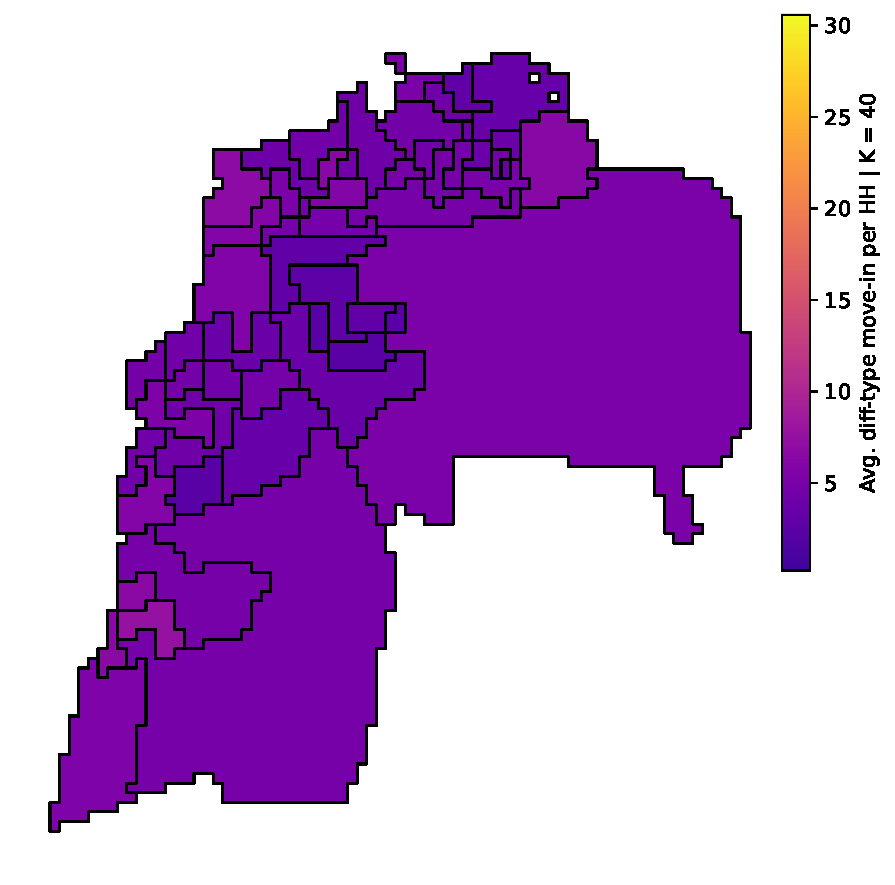
\includegraphics[width=\textwidth]{figs/ishoj_howdy_neighbor.pdf}	
	\caption{Ishøj}
	\end{subfigure}
    \begin{subfigure}{.42\textwidth}	
	\centering
	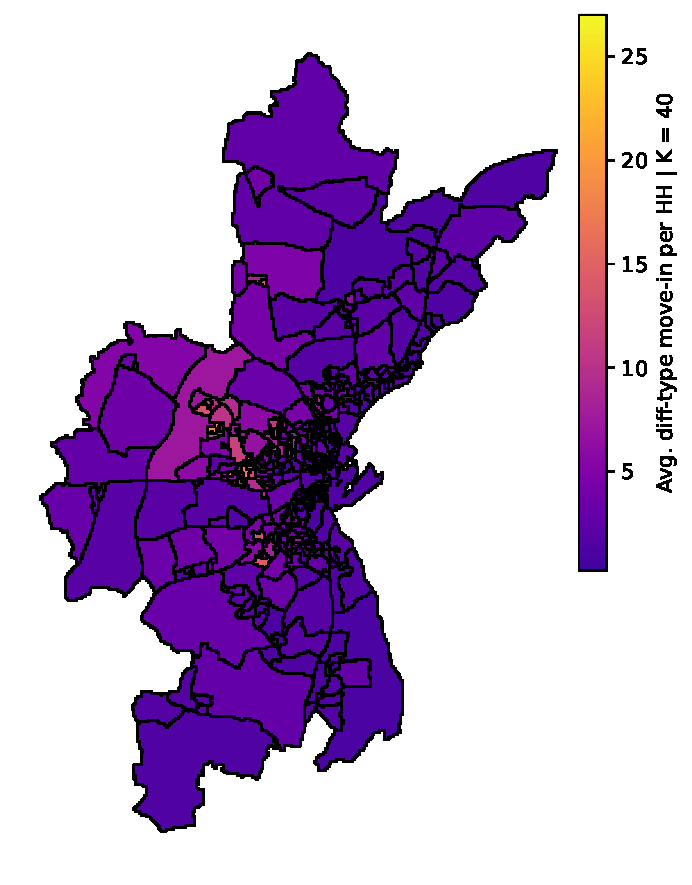
\includegraphics[width=\textwidth]{figs/aarhus_howdy_neighbor.pdf}	
	\caption{Aarhus}
	\end{subfigure}
    
    \begin{subfigure}{.65\textwidth}	
	\centering
	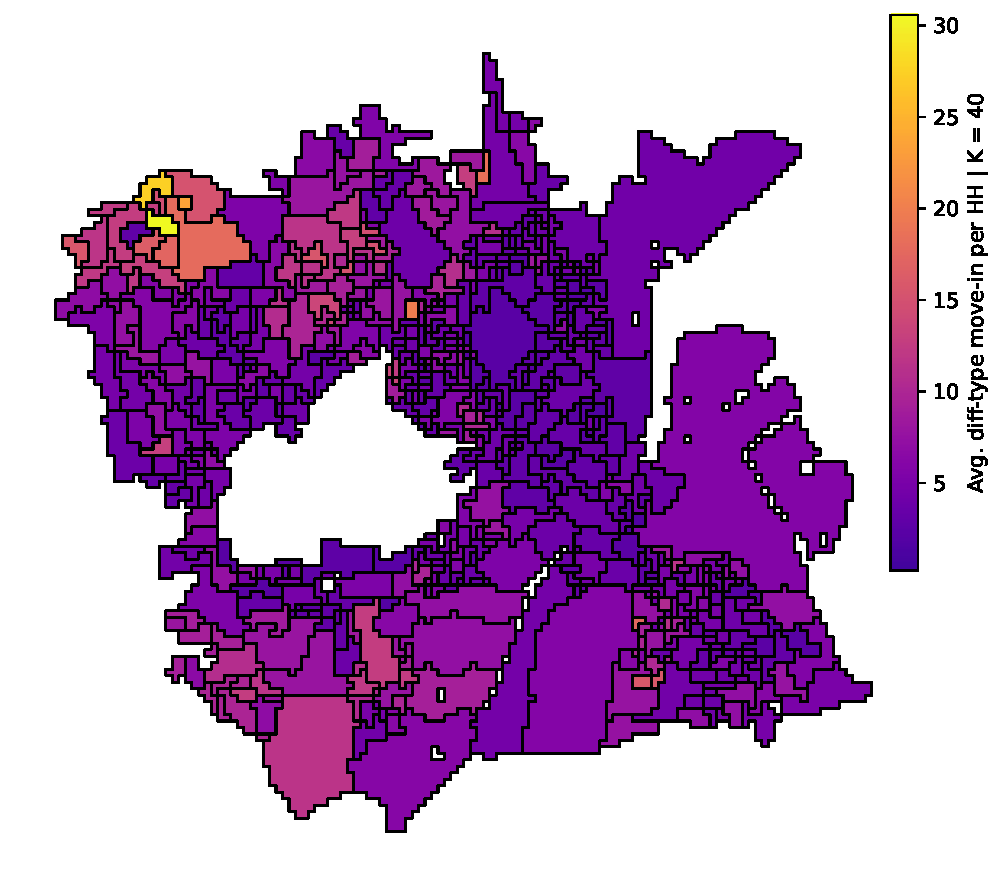
\includegraphics[width=\textwidth]{figs/cph_howdy_neighbor.pdf}	
	\caption{Copenhagen}
	\end{subfigure}	
\begin{tablenotes}[flushleft]
\item \footnotesize \textit{Note:} The figure show the variation in receiving a new-non West neighbor for native households at the \textit{neighborhood} scale for three different municipalities. Neighborhoods not in the sample are greyed out. Household types are split up in three types (native/non-West/West), see section \ref{sec:intro_definitions} for more details. Neighborhoods are defined in section \ref{sec:data_geospatial}. 
\end{tablenotes}
\label{fig:incidence_new_non_west_neighbors_unconstrained}
\end{figure}

\section{The Schelling Model}

\label{sec:appendix_schelling_model_simulation}

Consider a stylized example of Schelling's residential model: 
An $N \times N$ matrix $\textbf{M}$ represents possible residential locations. Two types of agents $b, r$, graphically depicted as blue and red, respectively, are initially allocated a random location within this grid. For the purpose of this paper, these differ in terms of ethnicity.

The ratio between the two types of agents is constant $N_{b/r} = \frac{N_b}{N_r}$. Further, a constant share of residential locations are vacant, such that $N_{vacant} = N^2 - (N_b + N_r)$. 

Each agent $i = b, r$ "optimizes" their residential location by how many of their $K$-nearest neighbors, $i_K$, are of the same type for some threshold $\tau$. That is, for $s_K \leq \tau$, where a $\tau$ is a fixed global tolerance parameter for the maximum share of neighbors of a different type, each agent $i$ will move until this condition is satisfied. In this very simple example, they move randomly to new vacant location at no cost. 

Below is a parameterization of the model described above such that red is always in the minority\footnote{This implementation closely follows \textcite{luca_mingarelli}, who very kindly made his code publicly available.}:

\begin{table}[H]
    \centering
    \caption{Schelling model parameters}
    \begin{tabular}{lc}
    \toprule
      Parameter & Value \\
    \midrule
      $N$         & 200 \\
      $N_{\frac{b}{r}}$       & 1.25 \\
      $N_{vacant}$ & 0.1 \\
    \bottomrule
    \end{tabular}
\end{table}

From here, we can perform element-wise multiplication and summation for each agent in $M$ to determine whether or not this satisfies the condition $s_i \leq \tau$. This process is called convolution and the operation can be done via the following kernel $\mathbf{K}$:

\newpage
\begin{lstlisting}[style=pythonstyle]
import numpy as np
KERNEL = np.array([[1,1,1,1,1],
                   [1,1,1,1,1],
                   [1,1,0,1,1],
                   [1,1,1,1,1],
                   [1,1,1,1,1]])

\end{lstlisting}

With the convolution operation defined as:

\begin{equation}
(K \star M)_{i, j}=\sum_{\substack{a \in\left\{-k_x, \ldots, k_x\right\} \\ b \in\left\{-k_y, \ldots, k_y\right\}}} K_{a+k_x, b+k_y} M_{i+a, j+b}
\label{eq:convolution}
\end{equation}

Where $k_x, k_y \in \mathbb{N}_0$. 


That is, I am considering the $k=24$ nearest neighbors in reference to the tolerance parameter $\tau$.

\begin{figure}[H]
\centering
\caption{Schelling model simulations by $\tau$ required same-type neighbors}
	\begin{subfigure}{0.45\textwidth}	
	\centering
    \caption{Integrated society, $\tau = 6$}
	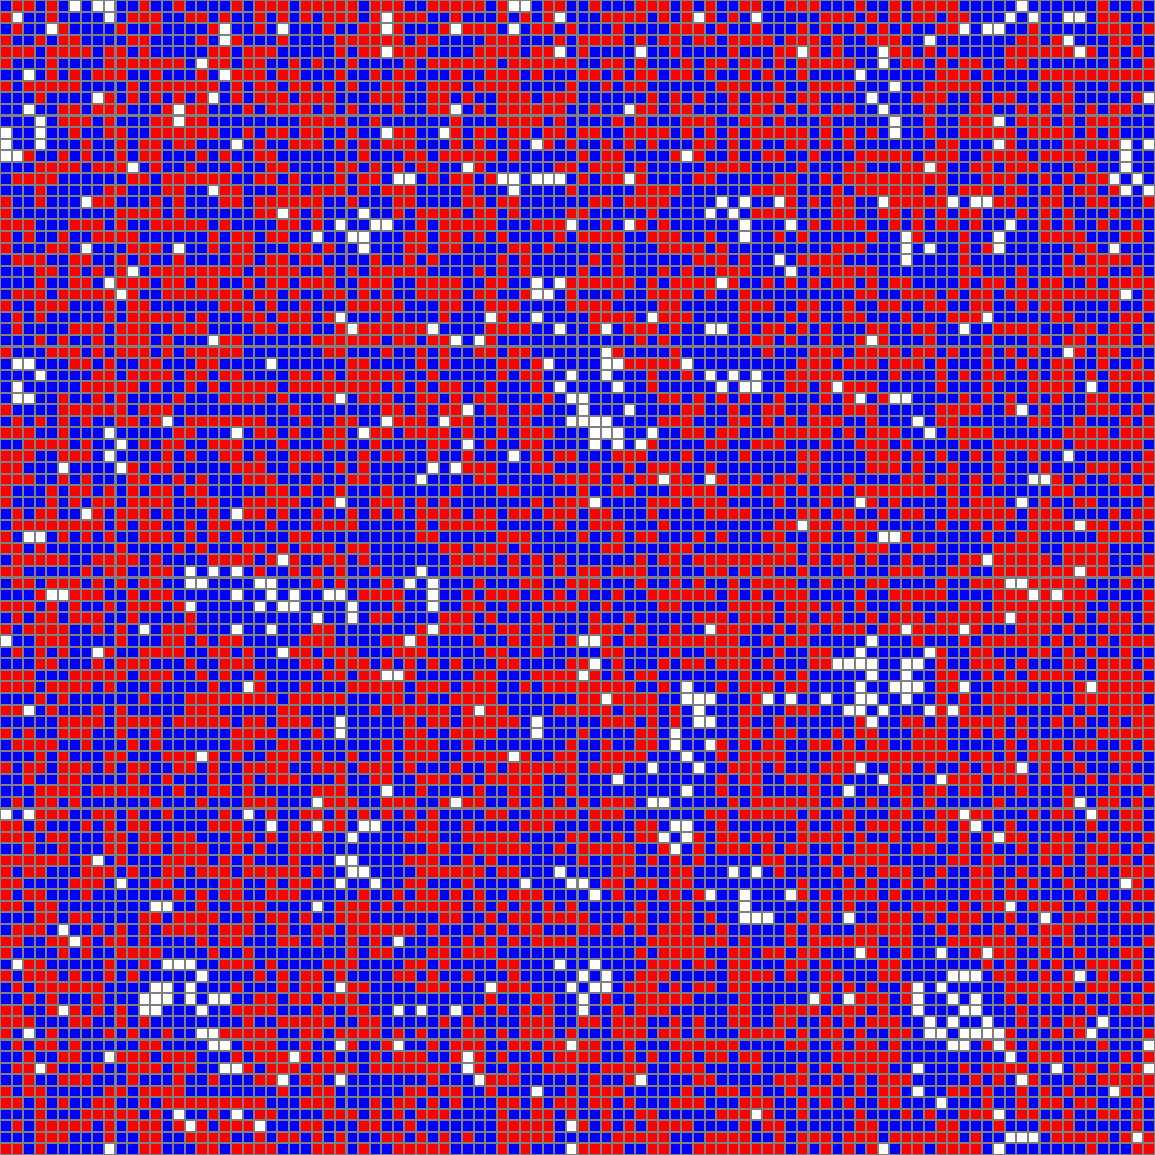
\includegraphics[width=\textwidth]{figs/schelling_6.pdf}	
	\end{subfigure}	
	\begin{subfigure}{0.45\textwidth}	
	\centering
    \caption{Inbetween society, $\tau = 8$}
	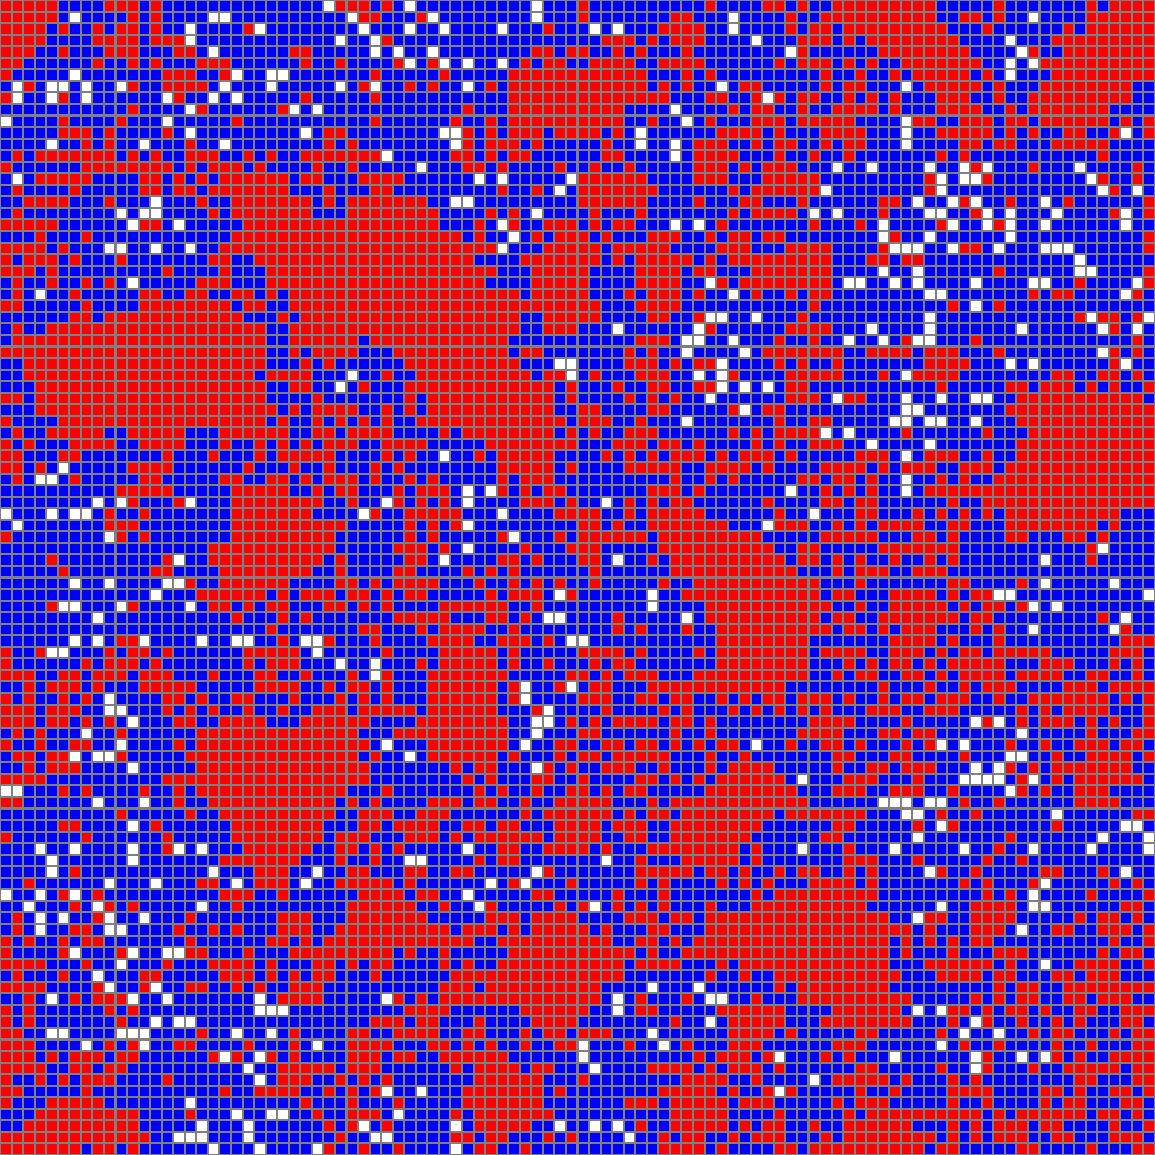
\includegraphics[width=\textwidth]{figs/schelling_8.pdf}	
	\end{subfigure}	
	\begin{subfigure}{0.45\textwidth}	
	\centering
     \caption{Segregated society, $\tau = 10$}
	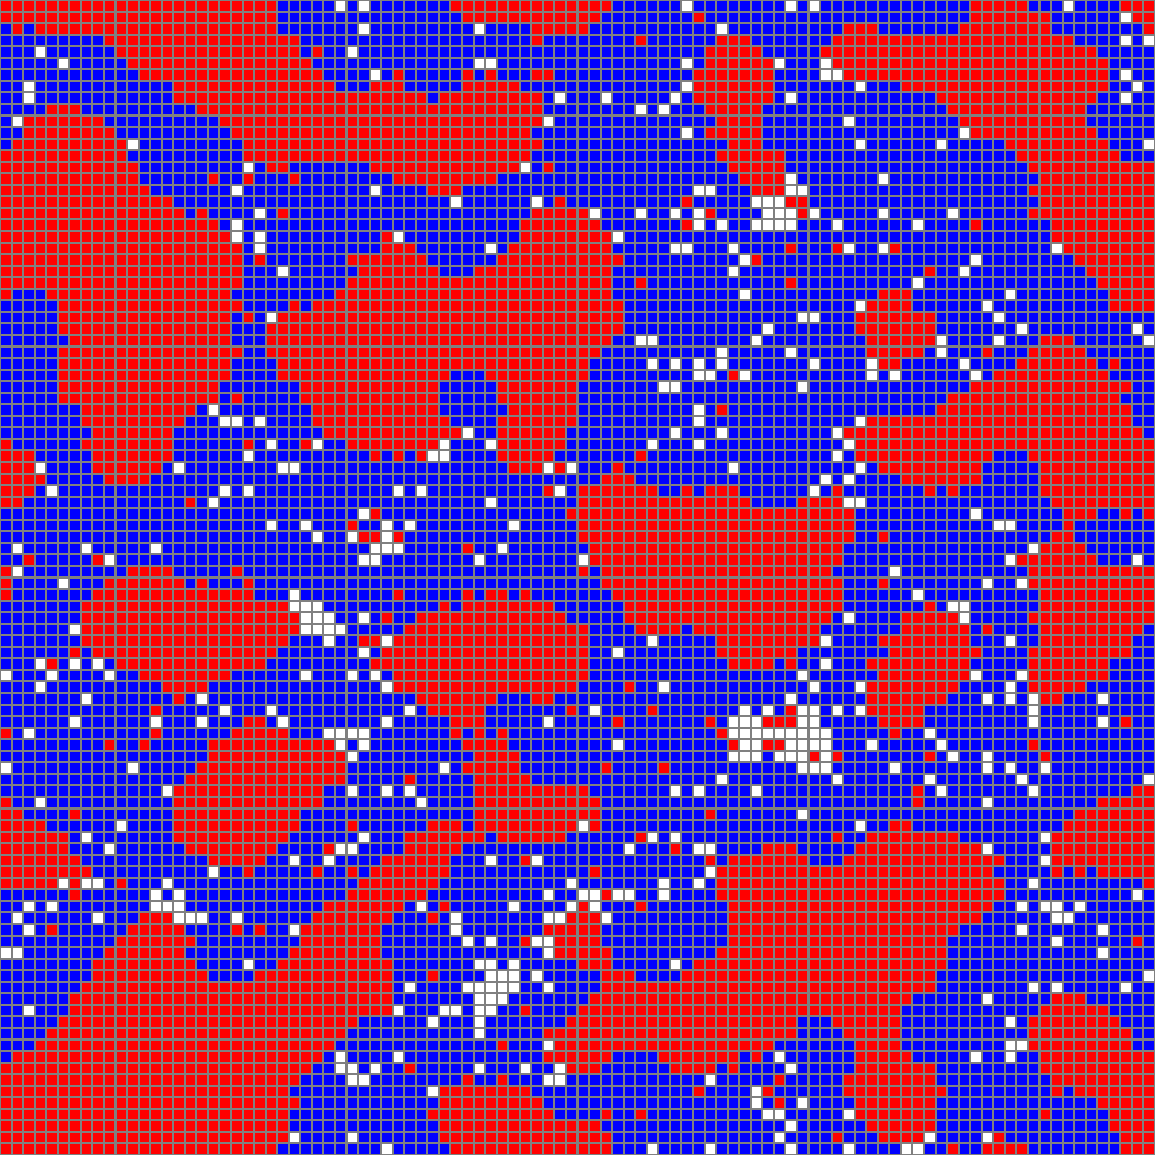
\includegraphics[width=\textwidth]{figs/schelling_10.pdf}	
	\end{subfigure}
    \begin{subfigure}{0.45\textwidth}	
	\centering
     \caption{"Gated" community, $\tau = 12$}
	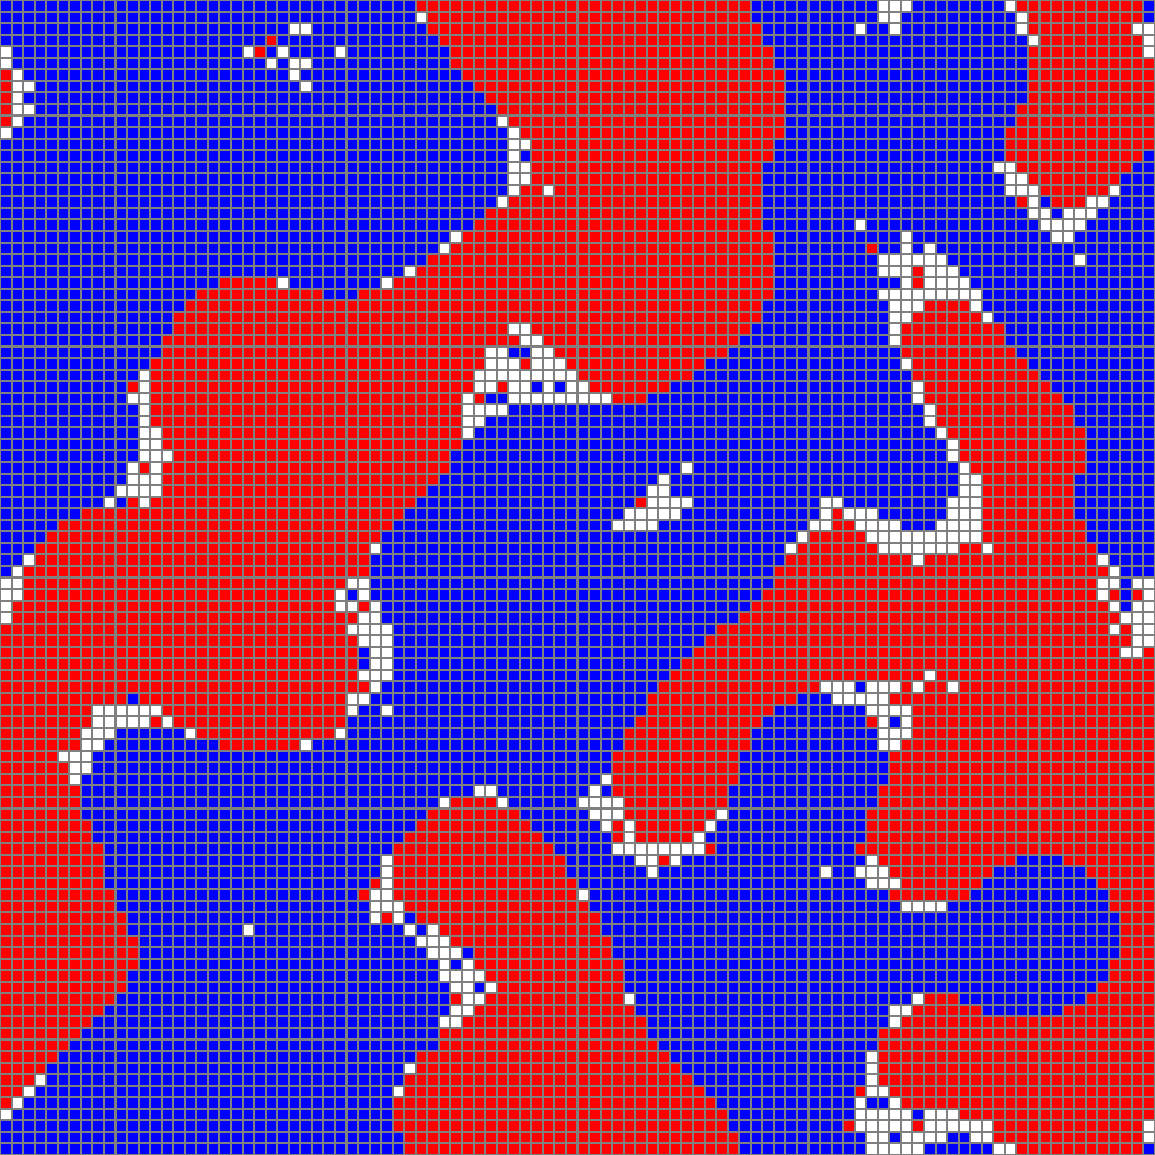
\includegraphics[width=\textwidth]{figs/schelling_12.pdf}	
	\end{subfigure}
\end{figure}

It is clear that the model predicts a segregated scenario for relatively mild preference parameters. Unsurprisingly, for sufficiently low levels of tolerances, one can observe fairly integrated societies. However, this pattern reverses once the tolerance parameter goes up, but not at levels one might expect. Even when agents are willing to accept up to 60 percent diverse neighbours ($1-\tau = 0.4$), we start to observe almost perfectly segregated societies.

...

\section{Random shit}
\label{sec:appendix_figs}
\begin{figure}[H]
    \centering
    \caption{Neighborhood population share by year}
    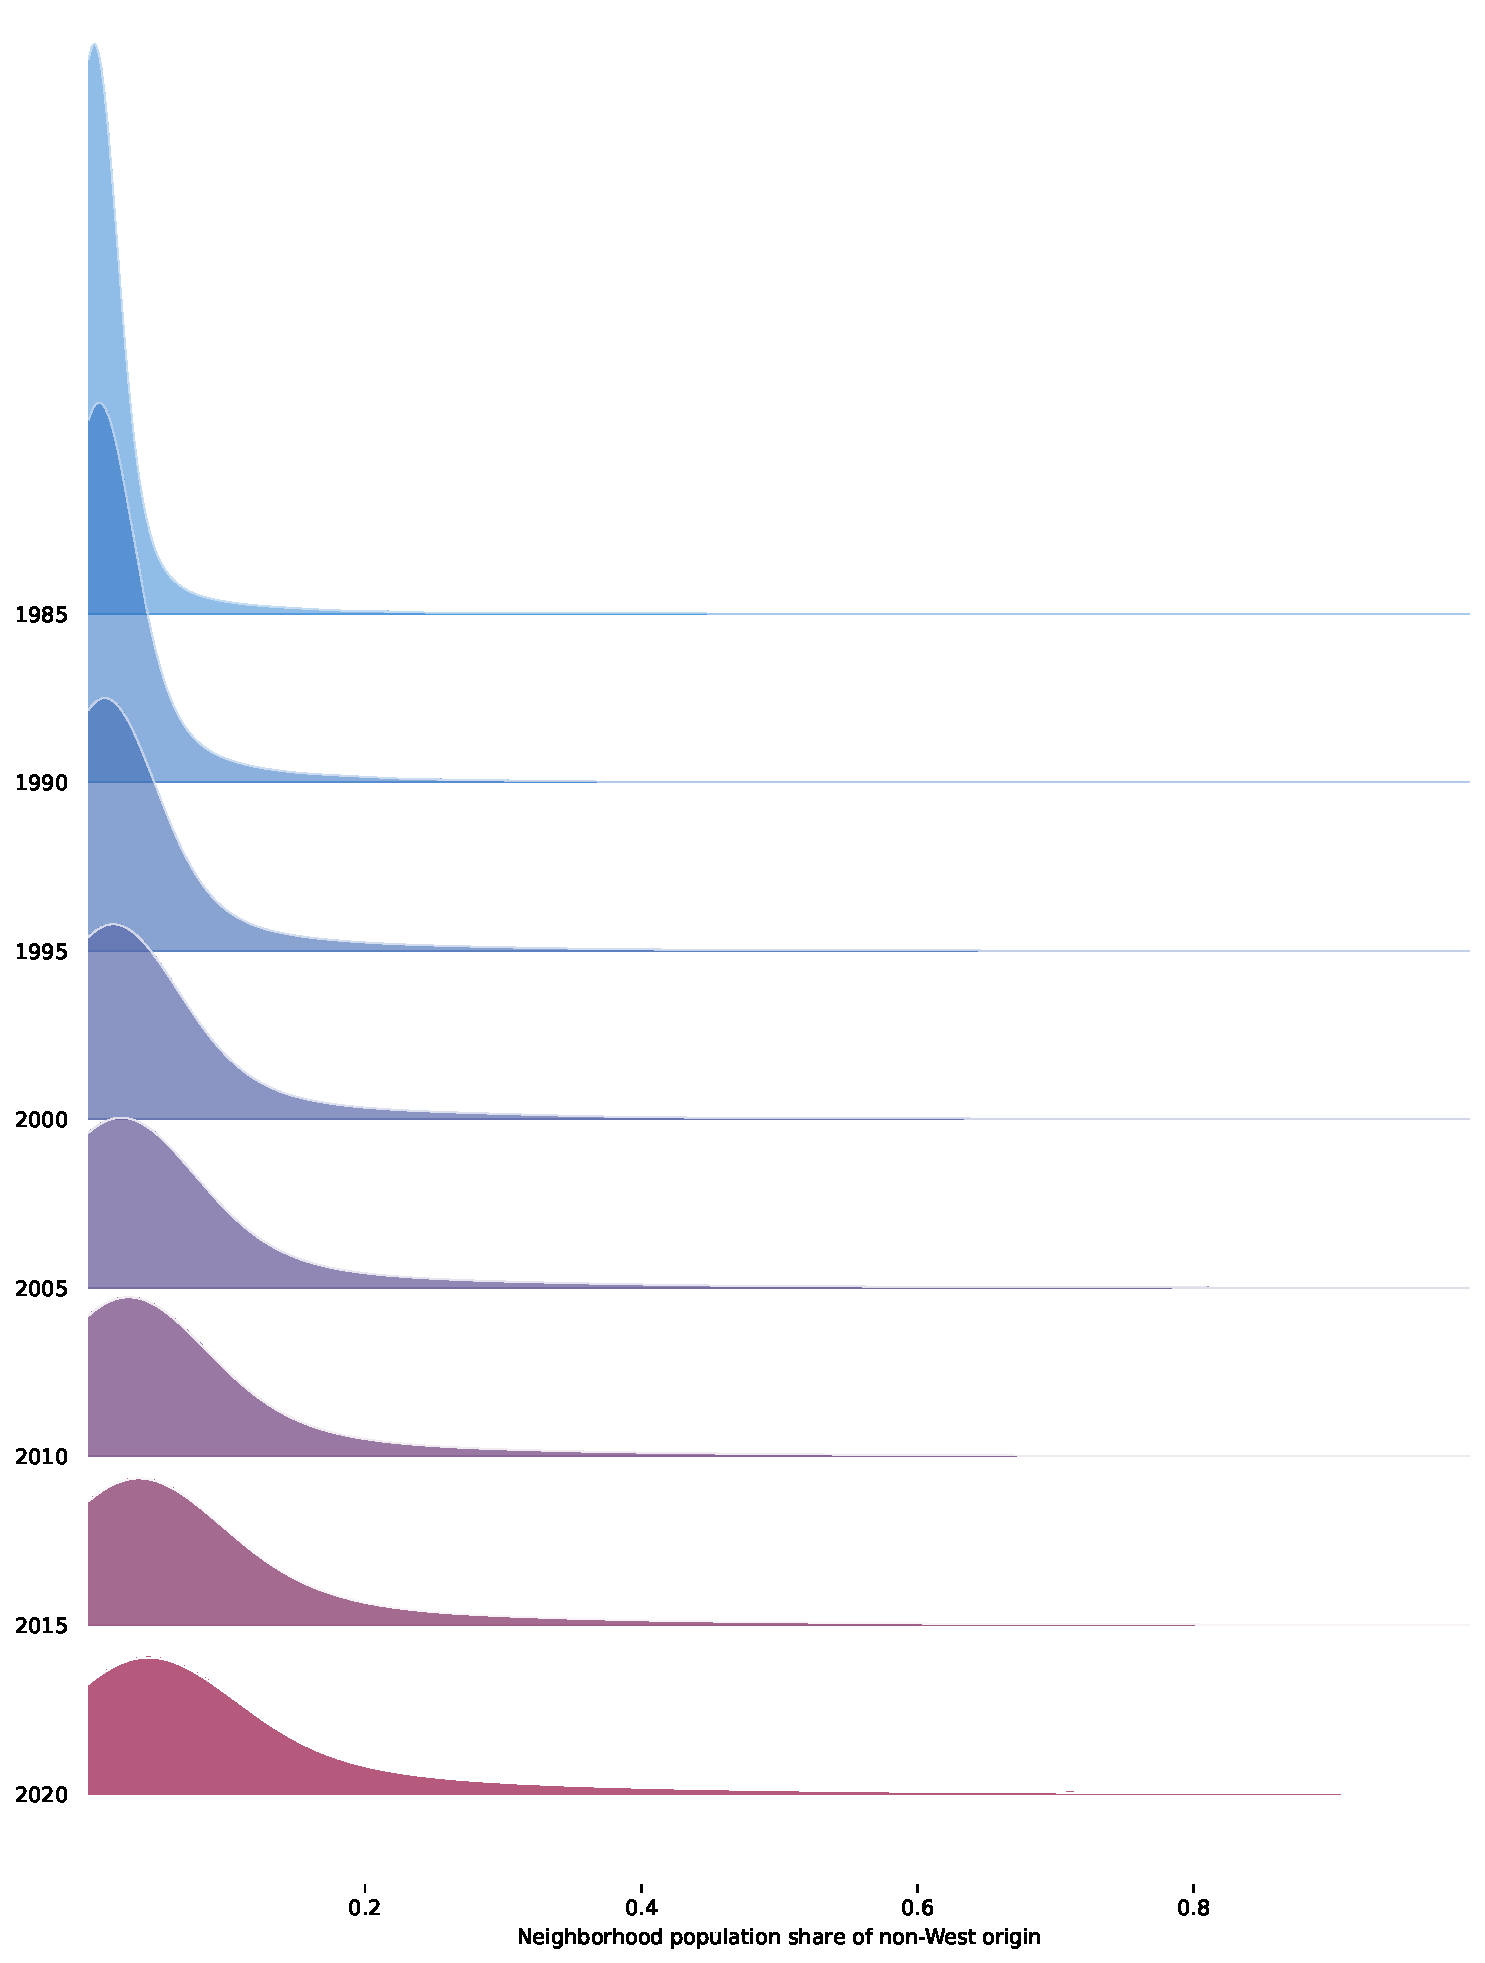
\includegraphics[width=0.7\linewidth]{figs/neighborhood_non_west_share_density_1985_2000.pdf}
        \begin{minipage}{.9\linewidth}
        \footnotesize \textit{Note}: Neighborhoods are derived from \href{https://www.nabolagsatlas.dk/}{Nabolagsatlas}. 
    \end{minipage}
\end{figure}

\begin{figure}[H]
    \centering
    \caption{K = 20 nearest }
    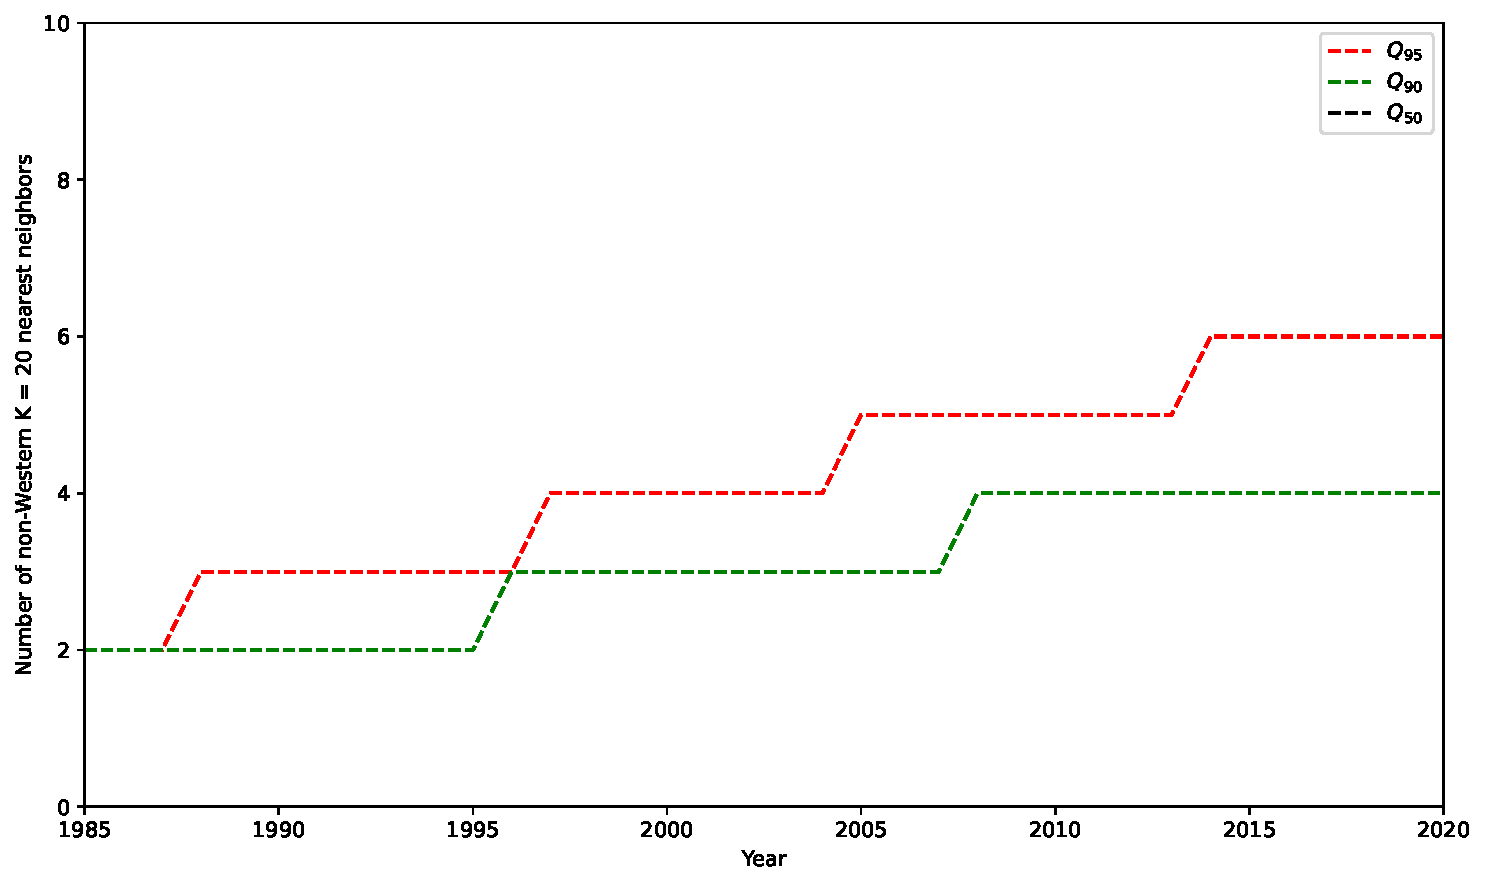
\includegraphics[width=0.7\linewidth]{figs/mix_non_west_pos_nn_quantiles_1985_2020.pdf}
        \begin{minipage}{.7\linewidth}
        \footnotesize \textit{Note}: Non-Western households refers to households where at least one household member is of non-Western origin.
    \end{minipage}
\end{figure}

\end{document}